Today, virtually all professional and open-source development teams use version control systems (VCSs) to manage changes in their projects.
StackOverflow reports over 96\% of professional developers use Git~\cite{vcs_usage}.
Git is a distributed VCS developed originally by Linus Torvalds and other contributors to the Linux kernel.
Version control systems enable developers to manage changes to code in their software projects.
A set of changes in Git is known as a commit~\cite{pro_git}.
Each commit points to one or more previous commits to form a tree (except for the first commit known as the root commit).
Multiple commits can have the same parent, which allows for a branching model and commits which have multiple parents merge two or more branches together.
\autoref{fig:git_branching} shows the Git branching model visually.

\begin{figure}[ht]
	\centering
	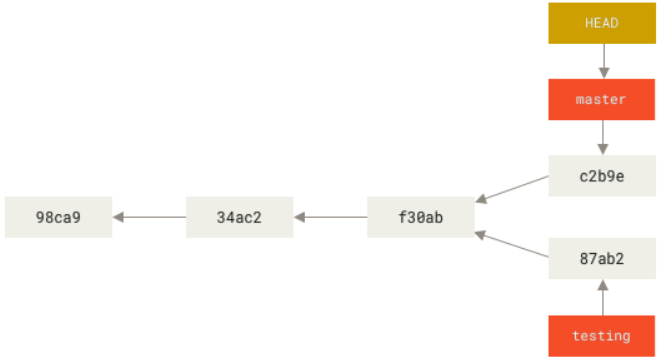
\includegraphics[width=0.35\textwidth]{images/git-branching}
	\caption{Git branching model, two branches exist one called master and one called testing~\cite{pro_git}.}
\label{fig:git_branching}
\end{figure}

Commits contain more information than just changes to file contents - they also include information about who authored the commit and who last applied it (for example, when a commit is imported from a patch file or when the commit is part of a rebase)---known as the author and committer respectively.
The field of mining software repositories (MSR) attempts to analyze the contents of software repositories to obtain useful information about a software project~\cite{road_ahead_for_msr}.

Code analysis tools are used to understand the quality of software code such as test coverage and security vulnerabilities.
Tools which do not run the code but instead analyse the code by reading it are called static code analysis.
One common type of static code analysis is static application security testing (SAST).
A SAST tool such a Snyk Code or SonarQube Security Analysis will analyze the code to detect common security vulnerabilities such as the use of known weak hashing or encryption algorithms, or known vulnerable dependency versions~\cite{scat}.
One common limitation of these tools, however, is that they only perform analysis on one version of the software.
It is possible then that an older version of the project used a dependency which has since had a vulnerability discovered---if the vulnerability is not present in a later version of the dependency (a version which the current version of the software project uses) then the SAST tool will not identify this vulnerability.
Similarly, as these tools continually improve and can detect more types of vulnerability it is possible that an older version of the project contains a vulnerability which was not initially discovered but running the tool again would result in it detecting the vulnerability.
This older version of the software could still be deployed, however and so identifying vulnerabilities in older versions of software is still important.

Another example of static code analysis is code coverage of software testing.
This type of tool will run tests written for the software and calculate the percentage of the program tested and which lines are untested.
While it could be useful for software development teams to see the trend in code coverage over time, code coverage tools typically only perform code coverage on the current version of the code.

A tool which performs analysis on multiple versions of the project could show a time-series graph to show how metrics change over time.
One example of this a graph which shows how the percentage of code covered by tests changes over time.

Iterating through each version of the project sequentially and running analysis is slow (the Linux repository for example has over 1.3m commits as of Dec 2022 and if each commit only took 1 second to be checked out and built it would still take 15 days to go through every commit~\cite{linux_git}).
Each version of the program does not depend on other versions previously having been built so parallelization can be used to significantly speed up this process.
Each process could use an isolated environment to avoid overwriting output from other processes.
